\documentclass[12pt,journal,compsoc]{IEEEtran}

\usepackage[portuguese]{babel}
\usepackage[utf8]{inputenc}
\usepackage{graphicx}
\usepackage[font=small,labelfont=bf]{caption}
\usepackage{breakurl}
\usepackage{color}

\begin{document}

\title{Análise comparativa de IDEs de programação Java: IntelliJ e Eclipse}
\author{
  Daniel~M.~Assis
  \IEEEcompsocitemizethanks{
    \IEEEcompsocthanksitem Daniel M. Assis (daniel.medeiros.assis@gmail.com)
  }
}

\IEEEcompsoctitleabstractindextext{%
\begin{abstract}
A produtividade é um dos aspectos mais importantes no desenvolvimento de softwares corporativos. Em uma realidade onde as empresas precisam cada vez mais entregar software com qualidade em prazos cada vez menores, as IDEs são ferramentas das mais importantes, provendo o programador com recursos valiosos para otimizar suas atividades. Este artigo apresenta um comparativo de duas das IDEs Java mais utilizadas no mercado pela ótica da produtividade do programador.
\end{abstract}
\begin{IEEEkeywords}
IDE, IntelliJ, Eclipse, Plugins, Produtividade, Java, Programação
\end{IEEEkeywords}}

\maketitle

\IEEEdisplaynotcompsoctitleabstractindextext
\IEEEpeerreviewmaketitle

\section{Introdução}

\IEEEPARstart{C}{a}da vez mais, na indústria de software, é preciso entregar novas funcionalidades e correções em tempo hábil e competitivo, ao mesmo tempo que uma grande ênfase à qualidade precisa ser observada. Um dos grandes desafios dos programadores de software é, portanto, realizar entregas de forma produtiva. Neste ínterim, o trabalho aqui proposto situa o programador de software em termos de seu papel na produtividade do projeto, e então, após demonstrar que esta produtividade está diretamente ligada ao uso de ferramentas IDE\cite{ide_definition}, apresenta um estudo comparativo das duas IDEs Java mais utilizadas no mercado. 

\section{As ferramentas e a produtividade}

A produtividade em programação refere-se a aspectos e metodologias de desenvolvimento de software que afetam a quantidade e qualidade do código-fonte produzido por um indivíduo ou time\cite{programming_productivity}. Existem vários aspectos a serem considerados, como quantidade de código, detecção e prevenção de erros, estimativa do custo de software, complexidade do sistema sendo construído. 

Banker e Kauffman\cite{measuring_productivity} sugerem que a medição de produtividade pode ser realizada por meio da relação entre o tamanho da aplicação e o trabalho consumido durante o desenvolvimento:

\begingroup
\fontsize{7pt}{8pt}\selectfont
\begin{verbatim}
Produtividade  =      Tamanho da aplicação desenvolvida
                 ------------------------------------------
                 Trabalho consumido durante desenvolvimento
\end{verbatim}
\endgroup

Nesta relação, faz-se evidente a importância da otimização do trabalho a ser realizado pelo programador de software, com consequências diretas na produtividade. Para esta otimização do esforço, são utilizadas ferramentas profissionais e especializadas.

\section{A IDE como ferramenta principal do programador}

Dentre as ferramentas mais utilizadas pelo programador de software, a IDE consolida-se como a principal, de acordo com a pesquisa "Developer Productivity Report 2013"\cite{zero_turnaround_2013}.

\begin{figure}[ht!]
\centering
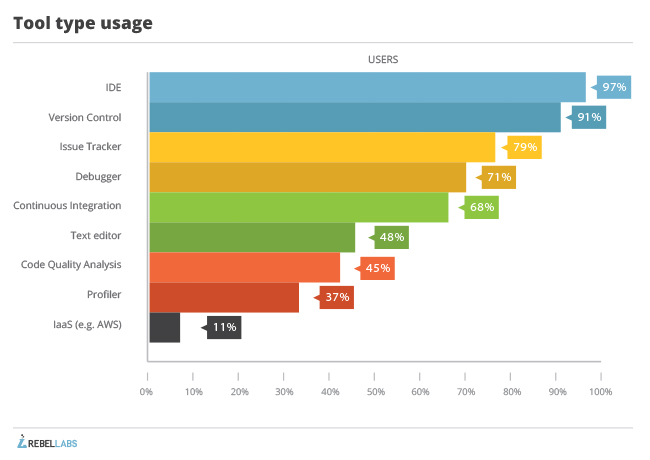
\includegraphics[width=0.5\textwidth]{img/16-tool-type-usage}
\caption{IDE é a ferramenta mais utilizada\cite{zero_turnaround_2013}}
\label{flow_before}
\end{figure}

Uma IDE é um programa de computador que reúne características e ferramentas de apoio ao desenvolvimento de software, visando agilizar o processo de desenvolvimento\cite{ide_definition}. Permite integrar diversas ações que são comuns aos desenvolvedores, como debug, edição, compilação, consulta à base de dados, dentre outras. Esta capacidade de reunir várias funcionalidades num único aplicativo é um aspecto de produtividade da IDE, contanto que as funcionalidades sejam consideradas úteis e satisfatórias pelos programadores. Há a possibilidade de uma dada IDE oferecer diversas funcionalidades que não sejam relevantes, de forma que nem sempre a IDE com mais itens deve ser considerada a melhor em termos de produtividade.

As duas IDEs mais utilizadas no mercado Java atualmente, conquistando a grande maioria da preferência dos programadores, são \emph{Eclipse} e \emph{IntelliJ} \cite{zero_turnaround}.

\begin{figure}[ht!]
\centering
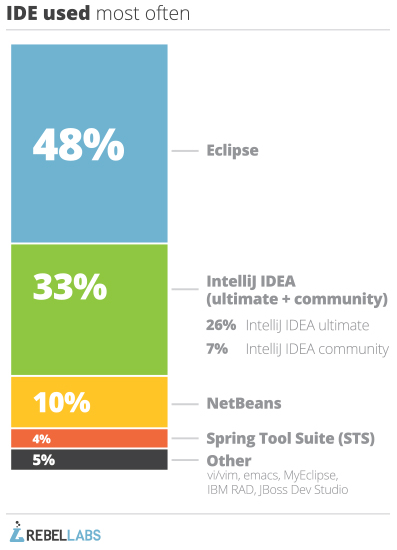
\includegraphics[width=0.5\textwidth]{img/ide-used-most-often-graph}
\caption{IDEs mais utilizadas \cite{zero_turnaround}}
\label{flow_before}
\end{figure}

Nesta mesma pesquisa, quando perguntados sobre \emph{"qual IDE você gostaria de utilizar ou testar para desenvolvimento"}, a preferência foi para o IntelliJ (em relação a qualquer outra IDE) \cite{zero_turnaround}.

\begin{figure}[ht!]
\centering
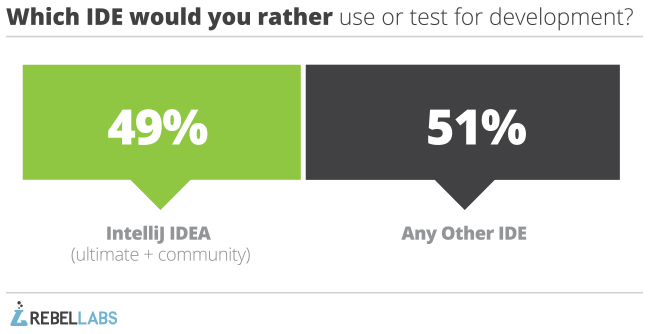
\includegraphics[width=0.5\textwidth]{img/which-ide-would-you-rather-use-or-test-for-development-graph}
\caption{IDEs preferidas para uso ou teste \cite{zero_turnaround}}
\label{flow_before}
\end{figure}


\section{Análise comparativa}

Uma vez estabelecido o papel da ferramenta IDE como sendo essencial para a produtividade do programador, o próximo passo é selecionar alguns critérios de comparação entre as IDEs. Numa pesquisa envolvendo dez programadores de software nível sênior, foram citados quinze funcionalidades como sendo as mais úteis que uma IDE pode apresentar. Cada uma destas funcionalidades foi analisada em ambas as IDEs (em máquinas Windows 7 com 8GB de RAM, e tendo por base alguns projetos multi-módulo de pequeno a grande porte), e as informações foram consolidadas em uma tabela comparativa, relacionando as duas IDEs em relação a cada uma das funcionalidades em questão. Ao mesmo tempo, um descritivo detalhado foi dado, para explicar a forma pela qual cada funcionalidade foi avaliada.

\subsection{Tabela Comparativa e Descritivo}

Segue abaixo a tabela que consolida as quinze funcionalidades em relação às IDEs. Exatamente um valor 'X' e um valor '-' são aplicados para cada critério, sendo o 'X' o indicador de que uma dada IDE é superior à sua concorrente, e o '-' o indicador de que a dada IDE é inferior à sua concorrente. O julgamento foi aplicado considerando tanto a opinião dos entrevistados quanto a verificação do pesquisador.

\begin{center}
  \begin{tabular}{| p{5cm} | c | c |}
    \hline
    Item & Eclipse & IntelliJ \\ 
    \hline
    Velocidade & -- & X \\  \hline
    Curva de Aprendizado & X & -- \\ \hline
    Suporte a Plugins & -- & X \\ \hline
    Estabilidade de Plugins & -- & X \\ \hline
    Estabilidade da IDE & -- & X \\ \hline
    Análise de Logs & -- & X \\ \hline
    Suporte à melhoria de qualidade & -- & X \\ \hline
    Diff de código & -- & X \\ \hline
    Integração com AppServer & -- & X \\ \hline
    Edição de Resource Bundles & -- & X \\ \hline
    Bind entre código Java e não-Java & -- & X \\ \hline
    Debug de JavaScript & -- & X \\ \hline
    Integração de Entidades com Bancos de Dados & -- & X \\ \hline
    Múltiplos projetos & X & -- \\ \hline
    Custo & X & -- \\ \hline
    \end{tabular}
\end{center}

\emph{Velocidade}: relativo à quanto tempo uma IDE demora em atividades que bloqueiam o programador. Observou-se lentidão no Eclipse em vários momentos, em projetos grandes, por conta de indexações feitas pelo plugin do Maven, validação de arquivos JavaScript, e outras causas não-aparentes; o desligamento destas funcionalidade é possível, mas nem sempre efetiva, em contraposição ao IntelliJ, que não apresentou nenhum problema de lentidão no mesmo ambiente e sob os mesmos projetos. Outra questão é a que o Eclipse trava em alguns momentos por razões não aparentes, mantendo uma tela branca por vários segundos, sendo necessário finalizar o processo e abrir a IDE novamente, em alguns casos; em nenhum momento, o IntelliJ apresentou travamento. Também sugere-se\cite{dropped_eclipse} que a velocidade de Debug do IntelliJ é superior ao Eclipse.

\emph{Curva de Aprendizado}: relativo a quanto esforço é gasto para aprender a IDE. O Eclipse ganha neste quesito, pelo fato de ser uma IDE mais conhecida pela maioria dos desenvolvedores Java. Ainda que programadores que utilizem IntelliJ sugiram que a curva de aprendizado é bem pequena, Eclipse tema vantagem de já ser mais conhecido.

\emph{Suporte a Plugins}: relativo à quantidade e qualidade dos plugins disponíveis para a IDE. Eclipse e IntelliJ tem, ambos, um suporte muito grande a plugins. Contudo, programadores entendem que o IntelliJ tem um melhor suporte, pois é comum que plugins no Eclipse, quando em grande quantidade, tornem a IDE mais lenta, que ofereçam travamento e que não funcionem da forma esperada (como no caso do plugin m2eclipse, para integração do Eclipse com Maven, que é algo extremamente importante mas não funciona de forma adequada); o IntelliJ não apresentou estes problemas.

\emph{Estabilidade de Plugins}: O IntelliJ ganha neste quesito pelo fato de a instalação de muitos plugins não ter ocasionado problemas de travamento ou lentidão perceptíveis. Tais problemas são comumente encontrados no Eclipse.

\emph{Estabilidade da IDE}: Pelo fato de ser comum no Eclipse o travamento e lentidão por razões diversas (impactando consideravelmente em produtividade), e por tais problemas não terem sido observados no IntelliJ em relação ao mesmo ambiente e aos mesmos projetos, o IntelliJ ganha neste quesito.

\emph{Análise de Logs}: O IntelliJ possui uma feature nativa que permite que um StackTrace seja copiado de um arquivo de Log e colado dentro da IDE, e então as classes que aparecem neste Log são diretamente mapeadas para classes do projeto aberto na IDE, de forma que basta clicar sobre a classe no log para a IDE abrir a classe Java diretamente na linha de código que apresenta problema. Esta funcionalidade é considerada extremamente útil pelos programadores, em especial em tarefas que envolvam rapidez em resolução, como atendimento a correção de bugs. O Eclipse não possui esta feature.

\emph{Suporte à melhoria de Qualidade}: relativo ao suporte da IDE para refatoração, testes automatizados e análise estática de código. Em relação à refatoração, observou-se que o IntelliJ é mais inteligente do que o Eclipse, no sentido que é mais capaz de inferir o que o programador quer, oferecendo opções mais adequadas.\cite{idea_better_eclipse} Sobre testes, IntelliJ possui a vantagem de autodetectar o tipo de framework (JUnit, TestNG) sendo utilizado e, a partir disto, executar propriamente (Eclipse precisa que a execução seja feita pelo plugin correspondente). Sobre análise estática de código, tanto IntelliJ quanto Eclipse possuem bons plugins para testes, mas IntelliJ sai na frente por possuir um plugin capaz de integrar FindBugs, PMD e Checkstyle, permitindo uma forma única de validar o código e importar regras de validação de ferramentas como o Sonar. O Eclipse lida com os plugins citados independentemente, de forma que a validação do código e a importação de regras faz-se mais trabalhosa. IntelliJ ainda dá feedback instantâneo, enquanto se digita código, através de warnings; no Eclipse, é preciso executar a análise manualmente (alguns plugins permitem a execução automática, mas só depois da classe ter sido salva).\cite{dropped_eclipse}.

\emph{Diff de código}: O IntelliJ possui a capacidade de exibir, no mesmo momento em que uma classe é modificada, qual era o estado anterior. Isto fica visível de forma muito simples: basta o programador colocar o mouse sobre uma barra lateral da classe para saber qual o estado anterior de linhas alteradas. Esta feature é considerada muito útil pelos desenvolvedores, que não se sentem intimidados pela quantidade de impacto que sua alteração está realizando. Além disto, também é possível, no IntelliJ, visualizar apenas os arquivos que foram alterados, e agrupar estes arquivos por assunto, o que facilita enormemente a realização de commits. No Eclipse, estas features não estão disponíveis.

\emph{Integração com AppServer}: relativo à capacidade da IDE de executar e testar a aplicação no servidor de aplicação, sem necessidade de realização do trabalho de forma externa à IDE. O Eclipse possui plugin para este trabalho, contudo, apresenta problemas, e seu uso é desencorajado pelos programadores, que preferem trabalhar com o Application Server por fora da IDE. Já no IntelliJ, as integrações com servidores de integração não apresentaram problemas, e funcionaram satisfatoriamente, sem ocasionar lentidão. Desta forma, o IntelliJ ganha neste quesito. Os Application Servers utilizados no teste foram Websphere e JBoss.

\emph{Edição de Resource Bundles}: relativo à capacidade de editar arquivos de propriedades da aplicação. No Eclipse, a edição é feita por meio de edição de texto simples. Já o IntelliJ oferece várias features para edição de arquivos deste tipo, tais como agrupamento de bundles por país, realização automática de Unicode e code complete, exibição de propriedades não sendo usadas na aplicação por meio de uma cor diferente que destaca-as das demais. Por isto, o IntelliJ ganhou neste quesito.

\emph{Bind entre código Java e não-Java}: relativo à capacidade de relacionar classes java com recursos não-Java. IntelliJ possui tal integração, sendo capaz de relacionar classes Java diretamente com outros tipos de arquivo (como JSP, por exemplo) que os referenciam. Este é um recurso muito prático para desenvolvimento de objetos Java em relação à camada de apresentação (e, inclusive, existe um grande suporte à sintaxe em diferentes linguagens, como Javascript, HTML, queries JPA, etc\cite{dropped_eclipse}). Esta feature existe de forma mais limitada no Eclipse.

\emph{Debug de JavaScript}: relativo à capacidade de Debugar arquivos JavaScript. Com IntelliJ, é possível realizar Debug de Javascript utilizando Chrome.

\emph{Integração de Entidades com Banco de Dados}: relativo ao bind entre entidades mapeadas por framework Objeto-Relacional e as tabelas de banco de dados que são mapeadas. O IntelliJ possui um recurso de autocomplete que permite, na edição da entidade, visualizar as colunas existentes na tabela, de forma a facilitar o trabalho de mapeamento. Tal recurso não encontra-se disponível no Eclipse.

\emph{Múltiplos Projetos}: Ainda que IntelliJ tenha a capacidade de abrir vários projetos (por meio do plugin do Maven), esta funcionalidade não é intuitiva. Já o Eclipse permite a abertura de projetos em "Workspaces", e cada Workspace ainda pode ter "Working Sets", para agrupamento dos projetos. Eclipse é melhor neste quesito.

\emph{Custo}: O Eclipse é uma ferramenta gratuita; já o Intellij é pago, com o valor da licença em 199 dólares para individual e 499 dólares para empresa (dados de setembro/2014). Eclipse ganha neste quesito.

\section{Relatório de produtividade com IntelliJ}

Uma feature nativa bastante interessante do IntelliJ é a possibilidade de medir a produtividade. O programador pode visualizar como está utilizando a IDE, de forma a poder melhorar sua própria produtividade pela otimização do uso da ferramenta. IntelliJ mantém um histórico de todas as ações e coleta as estatísticas, que são convertidas num relatório para análise. \cite{intellij_as_eclipse_user}

\begin{figure}[ht!]
\centering
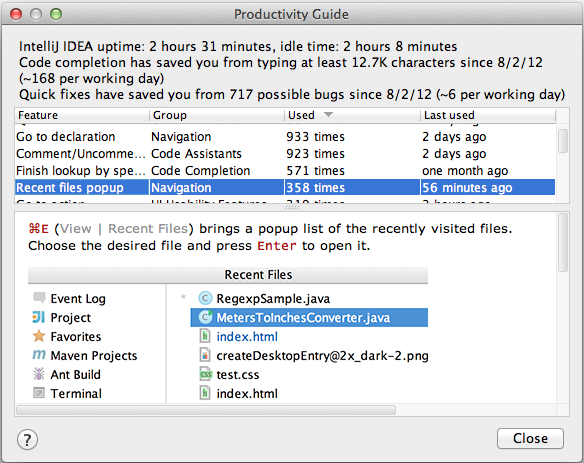
\includegraphics[width=0.5\textwidth]{img/54-productivity-guide}
\caption{Relatório de Produtividade do IntelliJ \cite{intellij_as_eclipse_user}}
\label{flow_before}
\end{figure}

\section{Considerações Finais}
Quando sugere-se que uma determinada feature não existe em uma IDE, parte-se do pressuposto que não existe a funcionalidade nativa e nem um plugin que a implemente e que funcione de forma satisfatória. Esta definição partiu do conhecimento dos entrevistados, que são programadores que atuam ou já atuaram com Eclipse e IntelliJ, bem como de pesquisas realizadas online. 

Outros aspectos ficaram de fora da pesquisa mas que merecem destaque são: detecção automática de frameworks (facets automáticos), autosave, falta de perspectives, chained completion, live templates.\cite{intellij_as_eclipse_user}

\section{Conclusão}
Este artigo demonstrou a importância da IDE como ferramenta de programação de software dentro do contexto de produtividade e, a partir desta definição, realizou uma análise comparativa de duas das IDEs preferidas do mercado. A premissa é que uma boa IDE faz o programador mais produtivo, contudo o conceito é subjetivo na medida em que a produtividade depende das funcionalidades que o programador quer e precisa\cite{intellij_as_eclipse_user} - e, por isto, os critérios utilizados na análise partiram de uma pesquisa envolvendo programadores. 

Considerando tais critérios, observou-se que, a despeito da popularidade, o Eclipse ficou atrás do IntelliJ. Sob a ótica dos plugins, ainda que possa ser sugerido que o Eclipse, com um conjunto bem específico de plugins, possa equiparar-se ao IntelliJ em relação aos critérios utilizados, seria uma afirmativa subjetiva sem que houvesse a enumeração de todos estes plugins e seu devido teste, e ainda deveria ser considerado o fato de que o Eclipse apresenta instabilidade quando do uso de determinados plugins. Além disto, aspectos como "Estabilidade da IDE" e "Velocidade" não podem ser equiparados, visto que não se trata de uma opção para o desenvolvedor, e sim um design da própria ferramenta.


\bibliographystyle{IEEEtran}
\bibliography{paper-intellij-eclipse}

\end{document}

